\section{Code and pilot data}
Summary data from the first \num{1000} imaging data points of the HCHS have been published with \citep{Schlemm2022-he}  and form the basis for the hypotheses tested in this replication study.
We have implemented our prespecified analysis pipeline described above in R and Matlab, and applied it to this previous sample.
Data, code and results have been stored on GitHub (\url{https://github.com/csi-hamburg/HCHS_brain_states_RR}) und preserved on Zenodo.

Thus re-analysing data from \num{988} subjects, the separation between two high-occupancy and three low-occupancy brain states could be reproduced for all combinations of brain parcellation and confound regression strategies (\Cref{fig:separation}).

\begin{figure}
    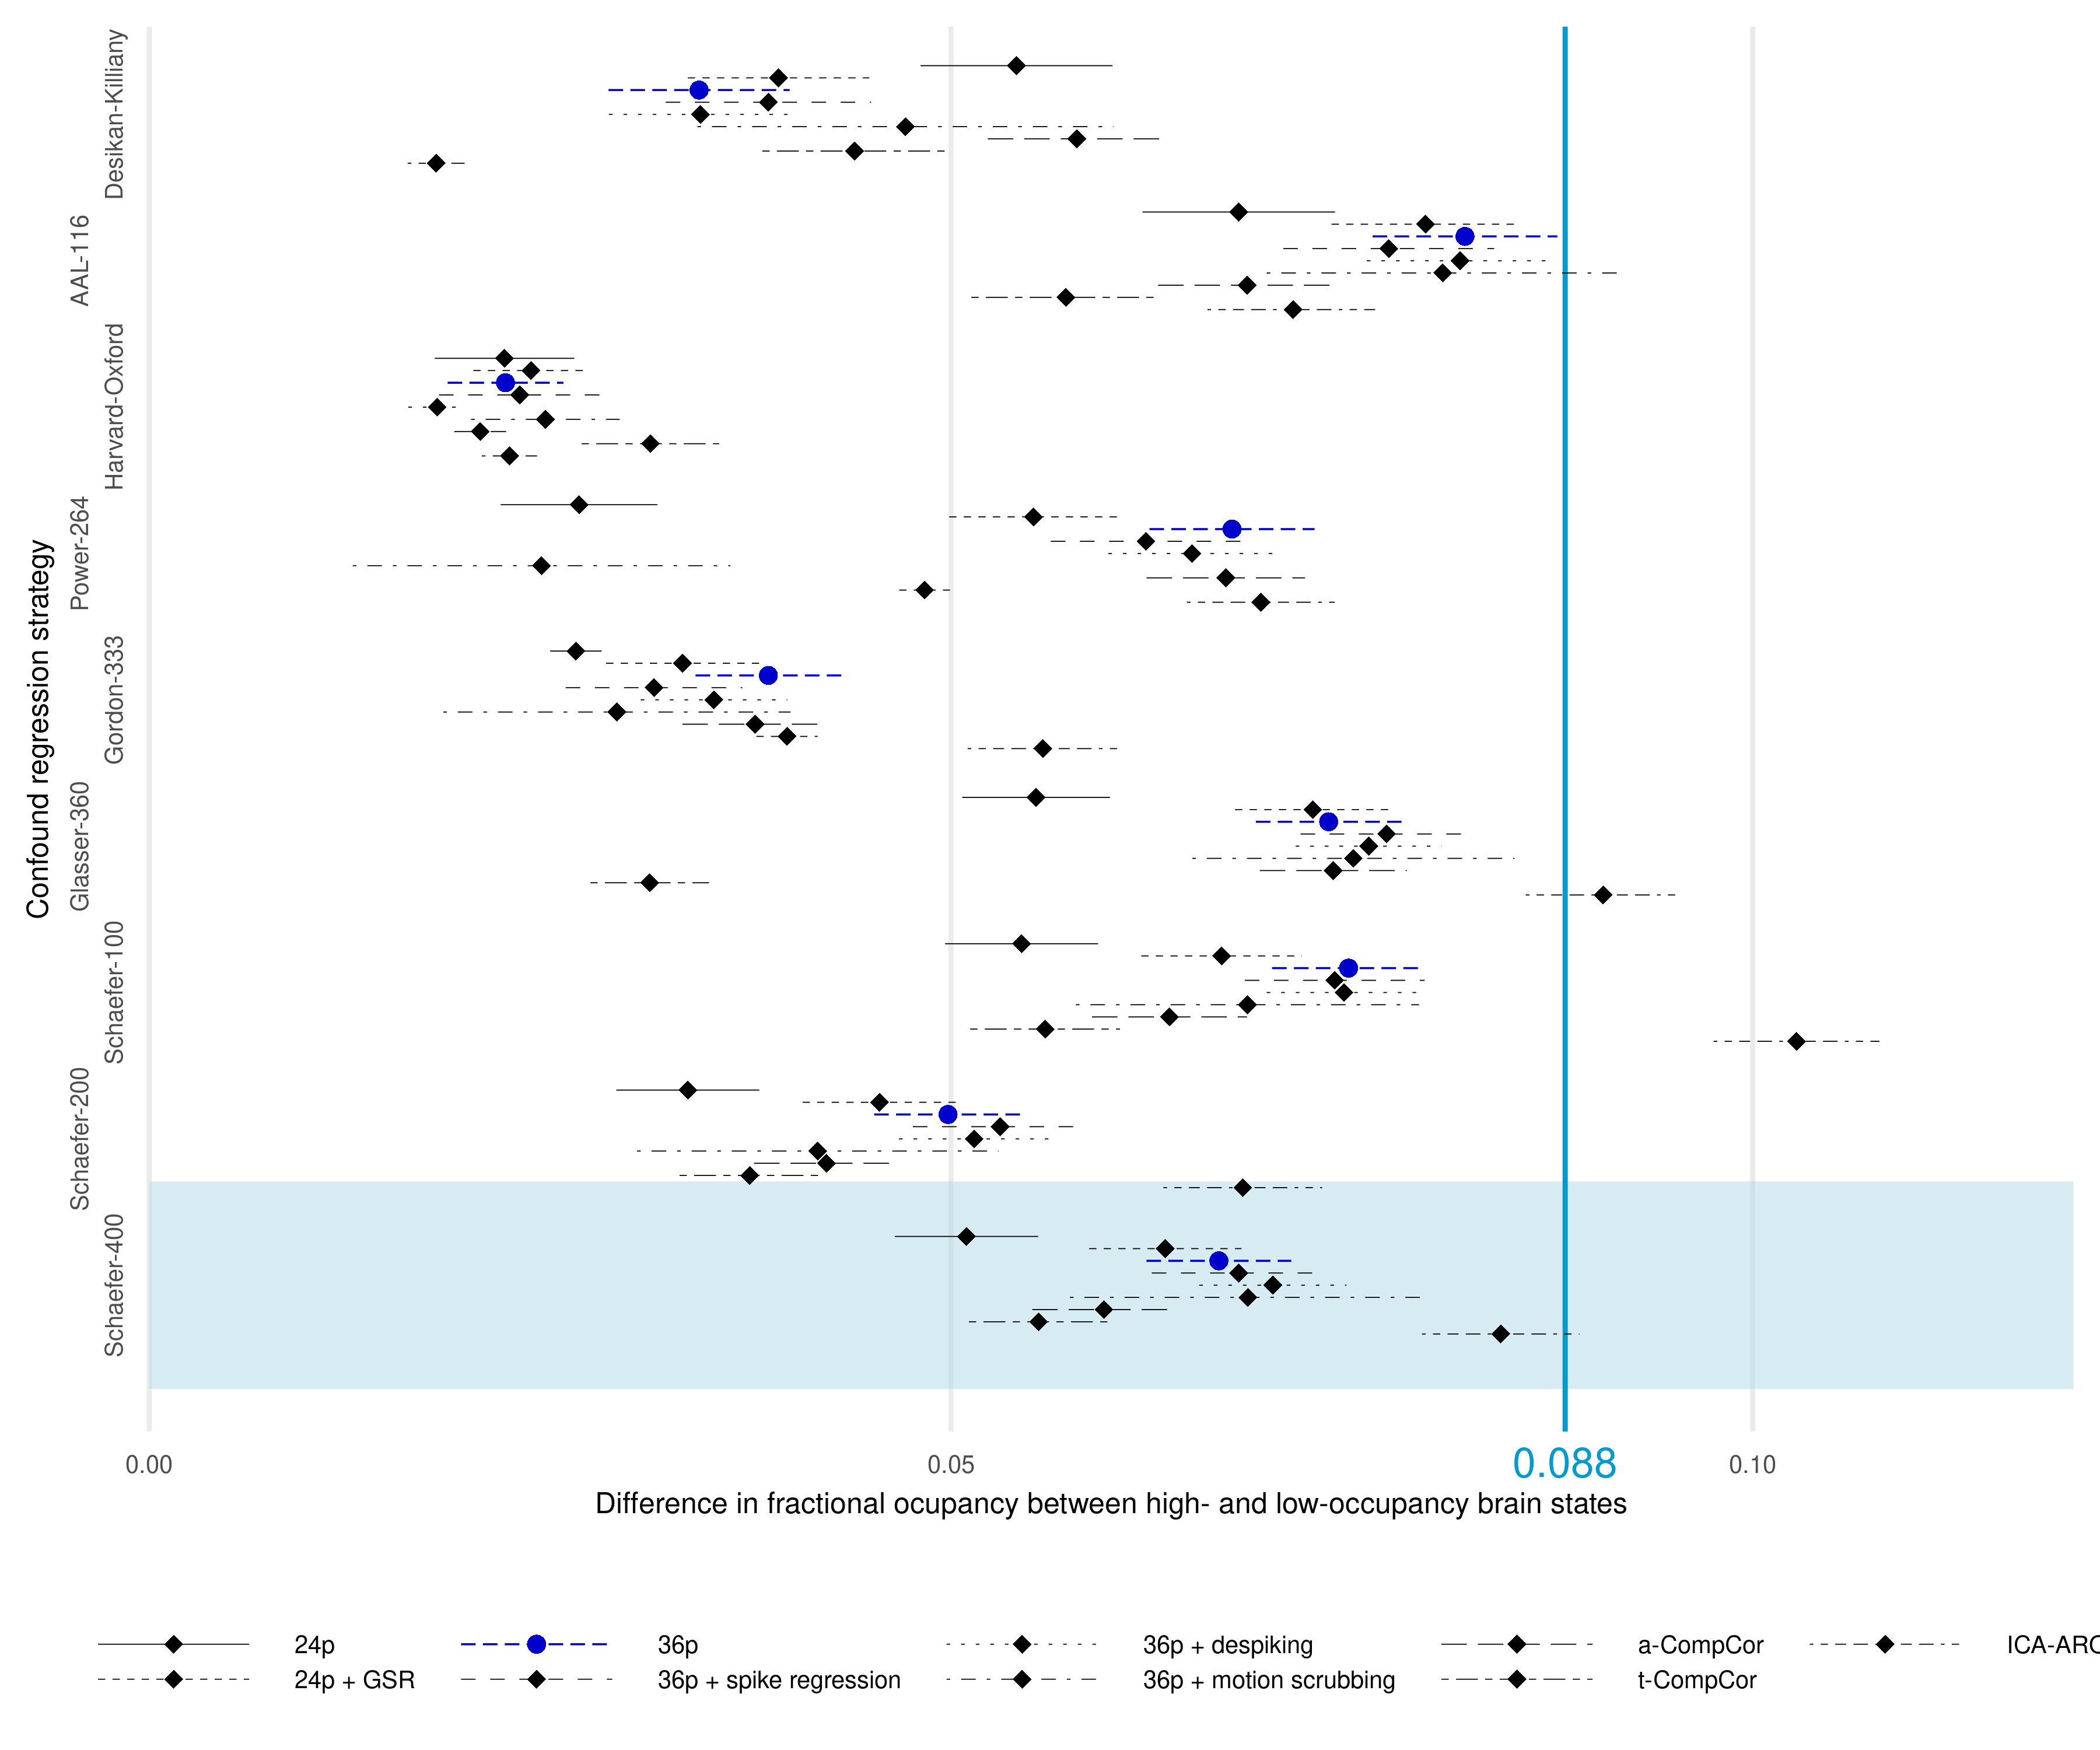
\includegraphics[width=\linewidth]{./../analysis/code/R/pipeline_files/figure-html/highVSlowFOplot-1.png}
    \caption{Point estimates and \qty{95}{\percent} confidence intervals for the mean in fractional occupancy between high- and low occupancy states are shown for different confound regression strategies and brain parcellations. The primary choices (\textit{36p} and \textit{schaefer400}) are highlighted by a yellow box and thick pink line, respectively. The effect size reported in \citep{Schlemm2022-he} is indicated by a vertical line at 0.08830623.}
    \label{fig:separation}
\end{figure}

In a multiverse analysis, the main finding was somewhat robust with respect to these choices: a statistically significant negative association between WMH load and time spent in high-occupancy states was observed in 18/81 scenarios, with 5/81 statistically significant positive associations occurring with the Desikan--Killiany parcellation only (\Cref{fig:refWMHvsFO}).

\begin{figure}
    \includegraphics[width=\linewidth]{./../analysis/code/R/pipeline_files/figure-html/regWMHvsFOplot-1.png}
    \caption{On the left, scatter plots of average fractional occupancies in high-occupancy states against WMH volume on a logarithmic scale (base 10 for easier visualization) for different combinations of confound regression strategies and brain parcellations. Linear regression lines indicate the direction of the unadjusted association between log(WMH) and occupancy. Background color of individual panels indicates the direction of the association after adjustment for age, sex and zero WMH volume (green, negative; red, positive). A pale background indicates that the association between log(WMH) and average occupancy is not statistically different from zero. On the right, the same information is shown using point estimates and \qty{95}{\percent} confidence intervals for the adjusted odds ratio of the association.}
    \label{fig:refWMHvsFO}
\end{figure}

The secondary finding of an association between greater TMT-B times and lower fractional occupancy was similarly robust with 12/81 statistically significant negative and no statistically significant positive associations.
